%%%%%%%%%%%%%%%%%%%%%%%%%%%%%%%%%%%%%%%%%%%%%%%%%%%%%%%%%%%%%%%%%%%%%%%%%%%%%%%%
% Modelo para artigo
%
% Por: Abrantes Araújo Silva Filho
%      abrantesasf@gmail.com


%%%%%%%%%%%%%%%%%%%%%%%%%%%%%%%%%%%%%%%%%%%%%%%%%%%%%%%%%%%%%%%%%%%%%%%%%%%%%%%%
%%% Classe do documento
\RequirePackage{ifpdf}
\ifpdf
  \documentclass[pdftex, brazil, 12pt, twoside]{article}
\else
  \documentclass[brazil, 12pt, twoside]{article}
\fi


%%%%%%%%%%%%%%%%%%%%%%%%%%%%%%%%%%%%%%%%%%%%%%%%%%%%%%%%%%%%%%%%%%%%%%%%%%%%%%%%
%%% Preâmbulo com todas as outras outras chamadas para todos os outros packages
%%% e o que mais for necessário
%%%%%%%%%%%%%%%%%%%%%%%%%%%%%%%%%%%%%%%%%%%%%%%%%%%%%%%%%%%%%%%%%%%%%%%%%%%%%%%%
% Por: Abrantes Araújo Silva Filho
%      abrantesasf@gmail.com
% URL: https://github.com/abrantesasf/latex


%%%%%%%%%%%%%%%%%%%%%%%%%%%%%%%%%%%%%%%%%%%%%%%%%%%%%%%%%%%%%%%%%%%%%%%%%%%%%%%%
%%% Compilação condicional em PDF
%%%%%%%%%%%%%%%%%%%%%%%%%%%%%%%%%%%%%%%%%%%%%%%%%%%%%%%%%%%%%%%%%%%%%%%%%%%%%%%%
% Por: Abrantes Araújo Silva Filho
%      abrantesasf@gmail.com
% URL: https://github.com/abrantesasf/latex


%%%%%%%%%%%%%%%%%%%%%%%%%%%%%%%%%%%%%%%%%%%%%%%%%%%%%%%%%%%%%%%%%%%%%%%%%%%%%%%%
%%% Pacote para compilaçãocondicional em PDF
\usepackage{ifpdf}


%%%%%%%%%%%%%%%%%%%%%%%%%%%%%%%%%%%%%%%%%%%%%%%%%%%%%%%%%%%%%%%%%%%%%%%%%%%%%%%%
%%% Estruturas de controle
%%%%%%%%%%%%%%%%%%%%%%%%%%%%%%%%%%%%%%%%%%%%%%%%%%%%%%%%%%%%%%%%%%%%%%%%%%%%%%%%
% Por: Abrantes Araújo Silva Filho
%      abrantesasf@gmail.com
% URL: https://github.com/abrantesasf/latex


%%%%%%%%%%%%%%%%%%%%%%%%%%%%%%%%%%%%%%%%%%%%%%%%%%%%%%%%%%%%%%%%%%%%%%%%%%%%%%%%
%%% Carrega pacotes iniciais necessários para estrutura de controle e para a
%%% criação e o parse de novos comandos
\usepackage{ifthen}
\usepackage{xparse}



%%%%%%%%%%%%%%%%%%%%%%%%%%%%%%%%%%%%%%%%%%%%%%%%%%%%%%%%%%%%%%%%%%%%%%%%%%%%%%%%
%%% Configurações de layout da página
%%%%%%%%%%%%%%%%%%%%%%%%%%%%%%%%%%%%%%%%%%%%%%%%%%%%%%%%%%%%%%%%%%%%%%%%%%%%%%%%
% Por: Abrantes Araújo Silva Filho
%      abrantesasf@gmail.com
% URL: https://github.com/abrantesasf/latex


%%%%%%%%%%%%%%%%%%%%%%%%%%%%%%%%%%%%%%%%%%%%%%%%%%%%%%%%%%%%%%%%%%%%%%%%%%%%%%%%
%%% Configuração do tamanho da página, margens, espaçamento entrelinhas e, se
%%% necessário, ativa a indentação dos primeiros parágrafos.
\makeatletter
\@ifclassloaded{beamer}{}{
\ifpdf
  \usepackage[pdftex]{geometry}
\else
  \usepackage[dvips]{geometry}
\fi
}
\makeatother

\usepackage{setspace}


%%%%%%%%%%%%%%%%%%%%%%%%%%%%%%%%%%%%%%%%%%%%%%%%%%%%%%%%%%%%%%%%%%%%%%%%%%%%%%%%
%%% Cabeçalho e rodapé
%%%%%%%%%%%%%%%%%%%%%%%%%%%%%%%%%%%%%%%%%%%%%%%%%%%%%%%%%%%%%%%%%%%%%%%%%%%%%%%%%
% Por: Abrantes Araújo Silva Filho
%      abrantesasf@gmail.com
% URL: https://github.com/abrantesasf/latex


%%%%%%%%%%%%%%%%%%%%%%%%%%%%%%%%%%%%%%%%%%%%%%%%%%%%%%%%%%%%%%%%%%%%%%%%%%%%%%%%
%%% Configurações de cabeçalho e rodapé:
%%% Atenção: é MUITO DIFÍCIL ajustar apropriadamente os running header
%%% e footer da primeira vez. Você pode confiar no LaTeX e deixar que
%%% ele faça o ajuste automaticamente ou pode quebrar a cabeça e
%%% tentar melhorar algo que o LaTeX já faz muito bem. O que você
%%% perfere?
\usepackage{fancyhdr}
\setlength{\headheight}{1cm}
\setlength{\footskip}{1.5cm}
\renewcommand{\headrulewidth}{0.3pt}
\renewcommand{\footrulewidth}{0.0pt}
\pagestyle{fancy}
\renewcommand{\sectionmark}[1]{%
  \markboth{\uppercase{#1}}{}}
\renewcommand{\subsectionmark}[1]{%
  \markright{\uppercase{\thesubsection \hspace{0.1cm} #1}}{}}
\fancyhead{}
\fancyfoot{}
\newcommand{\diminuifonte}{%
    \fontsize{9pt}{9}\selectfont
}
\newcommand{\aumentafonte}{%
    \fontsize{12}{12}\selectfont
}
% Configura cabeçalho e rodapé para documentos TWOSIDE
\fancyhead[EL]{\textbf{\thepage}}
\fancyhead[EC]{}
\fancyhead[ER]{\diminuifonte \textbf{\leftmark}}
\fancyhead[OR]{\textbf{\thepage}}
\fancyhead[OC]{}
\fancyhead[OL]{\diminuifonte \textbf{\rightmark}}
\fancyfoot[EL,EC,ER,OR,OC,OL]{}
% Configura cabeçalho e rodapé para documentos ONESIDE
%%\lhead{ \fancyplain{}{sup esquerdo} }
%%\chead{ \fancyplain{}{sup centro} }
%%\rhead{ \fancyplain{}{\thesection} }
%%\lfoot{ \fancyplain{}{inf esquerdo} }
%%\cfoot{ \fancyplain{}{inf centro} }
%%\rfoot{ \fancyplain{}{\thepage} }


%%%%%%%%%%%%%%%%%%%%%%%%%%%%%%%%%%%%%%%%%%%%%%%%%%%%%%%%%%%%%%%%%%%%%%%%%%%%%%%%
%%% Fontes
%%%%%%%%%%%%%%%%%%%%%%%%%%%%%%%%%%%%%%%%%%%%%%%%%%%%%%%%%%%%%%%%%%%%%%%%%%%%%%%%
% Por: Abrantes Araújo Silva Filho
%      abrantesasf@gmail.com
% URL: https://github.com/abrantesasf/latex


%%%%%%%%%%%%%%%%%%%%%%%%%%%%%%%%%%%%%%%%%%%%%%%%%%%%%%%%%%%%%%%%%%%%%%%%%%%%%%%%
%%% Configurações de encoding, lingua e fontes:
\usepackage[T1]{fontenc}
\usepackage[utf8]{inputenc}

% Altera a fonte padrão do documento (nem todas funcionam em modo math):
%   phv = Helvetica
%   ptm = Times
%   ppl = Palatino
%   pbk = bookman
%   pag = AdobeAvantGarde
%   pnc = Adobe NewCenturySchoolBook
\renewcommand{\familydefault}{ppl}


%%%%%%%%%%%%%%%%%%%%%%%%%%%%%%%%%%%%%%%%%%%%%%%%%%%%%%%%%%%%%%%%%%%%%%%%%%%%%%%%
%%% Linguagem e hifenização
%%%%%%%%%%%%%%%%%%%%%%%%%%%%%%%%%%%%%%%%%%%%%%%%%%%%%%%%%%%%%%%%%%%%%%%%%%%%%%%%
% Por: Abrantes Araújo Silva Filho
%      abrantesasf@gmail.com
% URL: https://github.com/abrantesasf/latex


%%%%%%%%%%%%%%%%%%%%%%%%%%%%%%%%%%%%%%%%%%%%%%%%%%%%%%%%%%%%%%%%%%%%%%%%%%%%%%%%
%%% Configurações de linguagem e hifenização
\usepackage[brazil]{babel}

%%%%%%%%%%%%%%%%%%%%%%%%%%%%%%%%%%%%%%%%%%%%%%%%%%%%%%%%%%%%%%%%%%%%%%%%%%%%%%%%
%%% Hifenização específica quando o LaTeX/Babel não conseguirem hifenizar:
\babelhyphenation{Git-Hub}


%%%%%%%%%%%%%%%%%%%%%%%%%%%%%%%%%%%%%%%%%%%%%%%%%%%%%%%%%%%%%%%%%%%%%%%%%%%%%%%%
%%% Matemática
%%%%%%%%%%%%%%%%%%%%%%%%%%%%%%%%%%%%%%%%%%%%%%%%%%%%%%%%%%%%%%%%%%%%%%%%%%%%%%%%
% Por: Abrantes Araújo Silva Filho
%      abrantesasf@gmail.com
% URL: https://github.com/abrantesasf/latex


%%%%%%%%%%%%%%%%%%%%%%%%%%%%%%%%%%%%%%%%%%%%%%%%%%%%%%%%%%%%%%%%%%%%%%%%%%%%%%%%
%%% Carrega bibliotecas e símbolos matemáticos, fontes adicionais e configura
%%% algumas outras opções
\usepackage{amsmath}
\usepackage{amssymb}
\usepackage{amsthm}
\usepackage{amsfonts}
\usepackage{siunitx}
  \sisetup{group-separator = {.}}
  \sisetup{group-digits = {true}}
  \sisetup{output-decimal-marker = {,}}
\usepackage{bm}
\usepackage{cancel}

% Altera separador decimal via comando, se necessário (prefira o siunitx):
%\mathchardef\period=\mathcode`.
%\DeclareMathSymbol{.}{\mathord}{letters}{"3B}

\usepackage{esvect}
\usepackage{mathtools}

%%%%%%%%%%%%%%%%%%%%%%%%%%%%%%%%%%%%%%%%%%%%%%%%%%%%%%%%%%%%%%%%%%%%%%%%%%%%%%%%
%%% Definições para teoremas, etc.
\makeatletter
\@ifclassloaded{article}{
\theoremstyle{definition}
\newtheorem{definicao}{Definição}[section]
\newtheorem{conjecture}{Conjectura}[section]
\newtheorem{teorema}{Teorema}[section]
\newtheorem{lemma}{Lema}[section]
\newtheorem{corolario}{Corolario}[section]
\theoremstyle{remark}
\newtheorem*{nota}{Nota}
\newtheorem*{observacao}{Observação:}
}{}
\@ifclassloaded{book}{
\theoremstyle{definition}
\newtheorem{definicao}{Definição}[chapter]
\newtheorem{conjecture}{Conjectura}[chapter]
\newtheorem{teorema}{Teorema}[chapter]
\newtheorem{lemma}{Lema}[chapter]
\newtheorem{corolario}{Corolario}[chapter]
\theoremstyle{remark}
\newtheorem*{nota}{Nota}
\newtheorem*{observacao}{Observação:}
}{}
\makeatother


%%%%%%%%%%%%%%%%%%%%%%%%%%%%%%%%%%%%%%%%%%%%%%%%%%%%%%%%%%%%%%%%%%%%%%%%%%%%%%%%
%%% Sumário
%%%%%%%%%%%%%%%%%%%%%%%%%%%%%%%%%%%%%%%%%%%%%%%%%%%%%%%%%%%%%%%%%%%%%%%%%%%%%%%%
% Por: Abrantes Araújo Silva Filho
%      abrantesasf@gmail.com
% URL: https://github.com/abrantesasf/latex


%%%%%%%%%%%%%%%%%%%%%%%%%%%%%%%%%%%%%%%%%%%%%%%%%%%%%%%%%%%%%%%%%%%%%%%%%%%%%%%%
%%% Ajustes de sumário
\makeatletter
\@ifclassloaded{article}{
\usepackage[nottoc]{tocbibind}
}{}
\@ifclassloaded{book}{
\usepackage{tocbibind}
}{}
\makeatother


%%%%%%%%%%%%%%%%%%%%%%%%%%%%%%%%%%%%%%%%%%%%%%%%%%%%%%%%%%%%%%%%%%%%%%%%%%%%%%%%
%%% Referências cruzadas, links, citações
%%%%%%%%%%%%%%%%%%%%%%%%%%%%%%%%%%%%%%%%%%%%%%%%%%%%%%%%%%%%%%%%%%%%%%%%%%%%%%%%
% Por: Abrantes Araújo Silva Filho
%      abrantesasf@gmail.com
% URL: https://github.com/abrantesasf/latex


%%%%%%%%%%%%%%%%%%%%%%%%%%%%%%%%%%%%%%%%%%%%%%%%%%%%%%%%%%%%%%%%%%%%%%%%%%%%%%%%%
%%% Carrega pacotes para referências cruzadas, citações dentro do documento,
%%% links para internet e outros.Configura algumas opções.
%%% Não altere a ordem de carregamento dos packages.
\usepackage{varioref}
\ifpdf
  \usepackage[pdftex]{hyperref}
    \hypersetup{
      % Configurações padrão que eu gosto
      unicode=true,
      pdflang={pt-BR},
      bookmarksopen=true,
      bookmarksnumbered=true,
      bookmarksopenlevel=5,
      pdfdisplaydoctitle=true,
      pdfpagemode=UseOutlines,
      pdfstartview=FitH,
      pdfcreator={LaTeX with hyperref package},
      pdfproducer={pdfTeX},
      pdfnewwindow=true,
      colorlinks=true,
      citecolor=red,
      linkcolor=red,
      filecolor=cyan,
      urlcolor=blue
    }
\else
  \usepackage{hyperref}
\fi
\usepackage{cleveref}
\usepackage{url}


%%%%%%%%%%%%%%%%%%%%%%%%%%%%%%%%%%%%%%%%%%%%%%%%%%%%%%%%%%%%%%%%%%%%%%%%%%%%%%%%
%%% Referências bibliográficas
%%%%%%%%%%%%%%%%%%%%%%%%%%%%%%%%%%%%%%%%%%%%%%%%%%%%%%%%%%%%%%%%%%%%%%%%%%%%%%%%
%%% Referências bibliográficas
\usepackage[round, semicolon, authoryear]{natbib}
%\bibliographystyle{natdin}
\bibliographystyle{abrantesasf}


%%%%%%%%%%%%%%%%%%%%%%%%%%%%%%%%%%%%%%%%%%%%%%%%%%%%%%%%%%%%%%%%%%%%%%%%%%%%%%%%
%%% Glossário e índice remissivo
%%%%%%%%%%%%%%%%%%%%%%%%%%%%%%%%%%%%%%%%%%%%%%%%%%%%%%%%%%%%%%%%%%%%%%%%%%%%%%%%
%%% Pacotes para glossário e índice remissivo
\usepackage{makeidx}
\makeindex

\usepackage[toc]{glossaries}
\newglossary[nlg]{notation}{not}{ntn}{Notação}

\newglossaryentry{not:set}{
type = notation,
name = {$\mathbb{N}$},
description = conjunto dos números naturais,
sort = {N}}

\makeglossaries


%%%%%%%%%%%%%%%%%%%%%%%%%%%%%%%%%%%%%%%%%%%%%%%%%%%%%%%%%%%%%%%%%%%%%%%%%%%%%%%%
%%% Computação
%%%%%%%%%%%%%%%%%%%%%%%%%%%%%%%%%%%%%%%%%%%%%%%%%%%%%%%%%%%%%%%%%%%%%%%%%%%%%%%%
% Por: Abrantes Araújo Silva Filho
%      abrantesasf@gmail.com
% URL: https://github.com/abrantesasf/latex


%%%%%%%%%%%%%%%%%%%%%%%%%%%%%%%%%%%%%%%%%%%%%%%%%%%%%%%%%%%%%%%%%%%%%%%%%%%%%%%%
%%% Carrega packages relacionados à computação
\usepackage{algorithm2e}
\usepackage{algorithmicx}
\usepackage{algpseudocode}
\usepackage{listings}
  \lstset{literate=
    {á}{{\'a}}1 {é}{{\'e}}1 {í}{{\'i}}1 {ó}{{\'o}}1 {ú}{{\'u}}1
    {Á}{{\'A}}1 {É}{{\'E}}1 {Í}{{\'I}}1 {Ó}{{\'O}}1 {Ú}{{\'U}}1
    {à}{{\`a}}1 {è}{{\`e}}1 {ì}{{\`i}}1 {ò}{{\`o}}1 {ù}{{\`u}}1
    {À}{{\`A}}1 {È}{{\'E}}1 {Ì}{{\`I}}1 {Ò}{{\`O}}1 {Ù}{{\`U}}1
    {ä}{{\"a}}1 {ë}{{\"e}}1 {ï}{{\"i}}1 {ö}{{\"o}}1 {ü}{{\"u}}1
    {Ä}{{\"A}}1 {Ë}{{\"E}}1 {Ï}{{\"I}}1 {Ö}{{\"O}}1 {Ü}{{\"U}}1
    {â}{{\^a}}1 {ê}{{\^e}}1 {î}{{\^i}}1 {ô}{{\^o}}1 {û}{{\^u}}1
    {Â}{{\^A}}1 {Ê}{{\^E}}1 {Î}{{\^I}}1 {Ô}{{\^O}}1 {Û}{{\^U}}1
    {œ}{{\oe}}1 {Œ}{{\OE}}1 {æ}{{\ae}}1 {Æ}{{\AE}}1 {ß}{{\ss}}1
    {ű}{{\H{u}}}1 {Ű}{{\H{U}}}1 {ő}{{\H{o}}}1 {Ő}{{\H{O}}}1
    {ç}{{\c c}}1 {Ç}{{\c C}}1 {ø}{{\o}}1 {å}{{\r a}}1 {Å}{{\r A}}1
    {€}{{\euro}}1 {£}{{\pounds}}1 {«}{{\guillemotleft}}1
    {»}{{\guillemotright}}1 {ñ}{{\~n}}1 {Ñ}{{\~N}}1 {¿}{{?`}}1
  }


%%%%%%%%%%%%%%%%%%%%%%%%%%%%%%%%%%%%%%%%%%%%%%%%%%%%%%%%%%%%%%%%%%%%%%%%%%%%%%%%
%%% Cores
%%%%%%%%%%%%%%%%%%%%%%%%%%%%%%%%%%%%%%%%%%%%%%%%%%%%%%%%%%%%%%%%%%%%%%%%%%%%%%%%
% Por: Abrantes Araújo Silva Filho
%      abrantesasf@gmail.com
% URL: https://github.com/abrantesasf/latex


%%%%%%%%%%%%%%%%%%%%%%%%%%%%%%%%%%%%%%%%%%%%%%%%%%%%%%%%%%%%%%%%%%%%%%%%%%%%%%%%
%%% Ativa suporte extendido a cores
\makeatletter
\@ifclassloaded{beamer}{
  \usepackage{xcolor} % Opções de cores: usenames (16), dvipsnames (64),
                      % svgnames (150) e x11names (300).
}{
  \usepackage[svgnames]{xcolor} % Opções de cores: usenames (16), dvipsnames (64),
                                % svgnames (150) e x11names (300).
}
\makeatother


%%%%%%%%%%%%%%%%%%%%%%%%%%%%%%%%%%%%%%%%%%%%%%%%%%%%%%%%%%%%%%%%%%%%%%%%%%%%%%%%
%%% Gráficos
%%%%%%%%%%%%%%%%%%%%%%%%%%%%%%%%%%%%%%%%%%%%%%%%%%%%%%%%%%%%%%%%%%%%%%%%%%%%%%%%
% Por: Abrantes Araújo Silva Filho
%      abrantesasf@gmail.com
% URL: https://github.com/abrantesasf/latex


%%%%%%%%%%%%%%%%%%%%%%%%%%%%%%%%%%%%%%%%%%%%%%%%%%%%%%%%%%%%%%%%%%%%%%%%%%%%%%%%
%%% Suporte à importação de gráficos externos
%\usepackage{tcolorbox}
\ifpdf
  \usepackage[pdftex]{graphicx}
\else
  \usepackage[dvips]{graphicx}
\fi

%%%%%%%%%%%%%%%%%%%%%%%%%%%%%%%%%%%%%%%%%%%%%%%%%%%%%%%%%%%%%%%%%%%%%%%%%%%%%%%%
%%% Suporte à criação de gráficos proceduralmente no LaTeX:
\usepackage{tikz}
\usetikzlibrary{arrows,automata,backgrounds,matrix,patterns,positioning,shapes,shadows}



%%%%%%%%%%%%%%%%%%%%%%%%%%%%%%%%%%%%%%%%%%%%%%%%%%%%%%%%%%%%%%%%%%%%%%%%%%%%%%%%
%%% Ícones
%%%%%%%%%%%%%%%%%%%%%%%%%%%%%%%%%%%%%%%%%%%%%%%%%%%%%%%%%%%%%%%%%%%%%%%%%%%%%%%%
% Por: Abrantes Araújo Silva Filho
%      abrantesasf@gmail.com
% URL: https://github.com/abrantesasf/latex


%%%%%%%%%%%%%%%%%%%%%%%%%%%%%%%%%%%%%%%%%%%%%%%%%%%%%%%%%%%%%%%%%%%%%%%%%%%%%%%%
%%% Pacotes com ícones, figuras e gráficos extras

% Ícones da Creative Commons:
\usepackage{ccicons}


%%%%%%%%%%%%%%%%%%%%%%%%%%%%%%%%%%%%%%%%%%%%%%%%%%%%%%%%%%%%%%%%%%%%%%%%%%%%%%%%
%%% Blocos
%%%%%%%%%%%%%%%%%%%%%%%%%%%%%%%%%%%%%%%%%%%%%%%%%%%%%%%%%%%%%%%%%%%%%%%%%%%%%%%%
% Por: Abrantes Araújo Silva Filho
%      abrantesasf@gmail.com
% URL: https://github.com/abrantesasf/latex


%%%%%%%%%%%%%%%%%%%%%%%%%%%%%%%%%%%%%%%%%%%%%%%%%%%%%%%%%%%%%%%%%%%%%%%%%%%%%%%%
%%% Ambiente para boxes em posições arbitrárias

\makeatletter
\@ifclassloaded{beamer}{
  \usepackage{textpos}
}{}
\makeatother


%%%%%%%%%%%%%%%%%%%%%%%%%%%%%%%%%%%%%%%%%%%%%%%%%%%%%%%%%%%%%%%%%%%%%%%%%%%%%%%%
%%% Boxes coloridos
%%%%%%%%%%%%%%%%%%%%%%%%%%%%%%%%%%%%%%%%%%%%%%%%%%%%%%%%%%%%%%%%%%%%%%%%%%%%%%%%
% Por: Abrantes Araújo Silva Filho
%      abrantesasf@gmail.com
% URL: https://github.com/abrantesasf/latex


%%%%%%%%%%%%%%%%%%%%%%%%%%%%%%%%%%%%%%%%%%%%%%%%%%%%%%%%%%%%%%%%%%%%%%%%%%%%%%%%
%%% Ativa suporte para boxes coloridos
\usepackage[most]{tcolorbox}


%%%%%%%%%%%%%%%%%%%%%%%%%%%%%%%%%%%%%%%%%%%%%%%%%%%%%%%%%%%%%%%%%%%%%%%%%%%%%%%%
%%% Tabelas
%%%%%%%%%%%%%%%%%%%%%%%%%%%%%%%%%%%%%%%%%%%%%%%%%%%%%%%%%%%%%%%%%%%%%%%%%%%%%%%%
% Por: Abrantes Araújo Silva Filho
%      abrantesasf@gmail.com
% URL: https://github.com/abrantesasf/latex


%%%%%%%%%%%%%%%%%%%%%%%%%%%%%%%%%%%%%%%%%%%%%%%%%%%%%%%%%%%%%%%%%%%%%%%%%%%%%%%%
%%% Packages para tabelas
\usepackage{array}
\usepackage{longtable}
\usepackage{tabularx}
\usepackage{tabu}
\usepackage{lscape}
\usepackage{colortbl}  
\usepackage{booktabs}


%%%%%%%%%%%%%%%%%%%%%%%%%%%%%%%%%%%%%%%%%%%%%%%%%%%%%%%%%%%%%%%%%%%%%%%%%%%%%%%%
%%% Ambientes de listas
%%%%%%%%%%%%%%%%%%%%%%%%%%%%%%%%%%%%%%%%%%%%%%%%%%%%%%%%%%%%%%%%%%%%%%%%%%%%%%%%
% Por: Abrantes Araújo Silva Filho
%      abrantesasf@gmail.com
% URL: https://github.com/abrantesasf/latex


%%%%%%%%%%%%%%%%%%%%%%%%%%%%%%%%%%%%%%%%%%%%%%%%%%%%%%%%%%%%%%%%%%%%%%%%%%%%%%%%
%%% Packages para ambientes de listas
\makeatletter
\@ifclassloaded{beamer}{
  \usepackage{listings}
}{
  \usepackage{enumitem}
  \usepackage[ampersand]{easylist}
}
\makeatother



%%%%%%%%%%%%%%%%%%%%%%%%%%%%%%%%%%%%%%%%%%%%%%%%%%%%%%%%%%%%%%%%%%%%%%%%%%%%%%%%
%%% Ambientes floats e similares
%%%%%%%%%%%%%%%%%%%%%%%%%%%%%%%%%%%%%%%%%%%%%%%%%%%%%%%%%%%%%%%%%%%%%%%%%%%%%%%%
% Por: Abrantes Araújo Silva Filho
%      abrantesasf@gmail.com
% URL: https://github.com/abrantesasf/latex


%%%%%%%%%%%%%%%%%%%%%%%%%%%%%%%%%%%%%%%%%%%%%%%%%%%%%%%%%%%%%%%%%%%%%%%%%%%%%%%%
%%% Packages para suporte a ambientes floats, captions, etc.:
\usepackage{float}
\usepackage{wrapfig}
\usepackage{placeins}
\usepackage{caption}
\usepackage{sidecap}
\usepackage{subcaption}


%%%%%%%%%%%%%%%%%%%%%%%%%%%%%%%%%%%%%%%%%%%%%%%%%%%%%%%%%%%%%%%%%%%%%%%%%%%%%%%%
%%% Meus comandos gerais
%%%%%%%%%%%%%%%%%%%%%%%%%%%%%%%%%%%%%%%%%%%%%%%%%%%%%%%%%%%%%%%%%%%%%%%%%%%%%%%%
% Por: Abrantes Araújo Silva Filho
%      abrantesasf@gmail.com
% URL: https://github.com/abrantesasf/latex


%%%%%%%%%%%%%%%%%%%%%%%%%%%%%%%%%%%%%%%%%%%%%%%%%%%%%%%%%%%%%%%%%%%%%%%%%%%%%%%%
%%% Vários comandinhos úteis e outras gambiarras

% Commando para ``italizar´´ palavras em inglês (e outras línguas!):
\newcommand{\ingles}[1]{\textit{#1}}

% Commando para colocar o espaço correto entre um número e sua unidade:
\newcommand{\unidade}[2]{\ensuremath{#1\,\mathrm{#2}}}
\newcommand{\unidado}[2]{{#1}\,{#2}}

% Produz ordinal masculino ou feminino dependendo do segundo argumento:
\newcommand{\ordinal}[2]{%
#1%
\ifthenelse{\equal{a}{#2}}%
{\textordfeminine}%
{\textordmasculine}}

% Comando para colocar o autor da citação corretamente justificado à direita:
% Modificado de: https://latex.org/forum/viewtopic.php?p=15605&sid=216895679326b531e85caec779e1d710#p15605
\newcommand*{\fontequote}[2]{%
   \unskip\hspace*{1em plus 1fill}%
   \linebreak\hspace*{\fill}\mbox{#1}\vspace{-0.15cm}
   \linebreak\hspace*{\fill}\mbox{#2}
}




%%%%%%%%%%%%%%%%%%%%%%%%%%%%%%%%%%%%%%%%%%%%%%%%%%%%%%%%%%%%%%%%%%%%%%%%%%%%%%%%
%%% Ajuste do layout, espaçamento de linhas e etc.:
\geometry{a4paper, left=2cm, right=2cm, top=2cm, bottom=2cm}
\onehalfspacing


%%%%%%%%%%%%%%%%%%%%%%%%%%%%%%%%%%%%%%%%%%%%%%%%%%%%%%%%%%%%%%%%%%%%%%%%%%%%%%%%
%%% Configurações para as propriedades do PDF:
\hypersetup{
      pdftitle={Integrais duplas em coordenadas polares},
      pdfauthor={Abrantes Araújo Silva Filho},
      pdfsubject={Integrais múltiplas},
      pdfkeywords={cálculo integral, integrais duplas, sistema de
        coordenadas polares},
      pdfinfo={
        CreationDate={}, % Ex.: D:AAAAMMDDHH24MISS
        ModDate={}       % Ex.: D:AAAAMMDDHH24MISS
      }}


%%%%%%%%%%%%%%%%%%%%%%%%%%%%%%%%%%%%%%%%%%%%%%%%%%%%%%%%%%%%%%%%%%%%%%%%%%%%%%%%
%%% Compilação condicional de capítulos
%\includeonly{}


%%%%%%%%%%%%%%%%%%%%%%%%%%%%%%%%%%%%%%%%%%%%%%%%%%%%%%%%%%%%%%%%%%%%%%%%%%%%%%%%
%%% Comandos específicos para este artigo
% Define o diferencial "d"
\newcommand*\diff{\mathop{}\!\mathrm{d}}
\newcommand*\Diff[1]{\mathop{}\!\mathrm{d^#1}}


%%%%%%%%%%%%%%%%%%%%%%%%%%%%%%%%%%%%%%%%%%%%%%%%%%%%%%%%%%%%%%%%%%%%%%%%%%%%%%%%
%%% Começa o documento
\begin{document}


%%%%%%%%%%%%%%%%%%%%%%%%%%%%%%%%%%%%%%%%%%%%%%%%%%%%%%%%%%%%%%%%%%%%%%%%%%%%%%%%
%%% Front matter
\title{Integrais duplas em coordenadas polares}
\author{Grupo 1}
\date{2019-11-08}
\maketitle

%\renewcommand{\abstractname}{novo título do abstract}
\abstract{Trabalho acadêmico sobre integrais duplas em coordenadas
  polares, apresentado na disciplina de \emph{Cálculo III} sob orientação do
  prof. Kennedy Scopel Gomes, como requisito parcial da terceira
  avaliação semestral.

  Aborda uma revisão rápida sobre o conceito de integrais e o cálculo
  de áreas e volumes, discute quando o cálculo de volumes com
  integrais duplas em coordenadas retangulares é difícil de ser
  realizado, e apresenta uma solução através da utilização de
  coordenadas polares.}

\tableofcontents


%%%%%%%%%%%%%%%%%%%%%%%%%%%%%%%%%%%%%%%%%%%%%%%%%%%%%%%%%%%%%%%%%%%%%%%%%%%%%%%%
%%% Main matter
\section{Revisão rápida}
\label{sec:revisao}

\subsection{Integrais simples e o cálculo de áreas}
\label{sec:revisao-int1}
Um dos problemas fundamentais do cálculo é a determinação da \emph{área} sob
uma uma função $y = f(x)$ qualquer, quando $x$ varia em um intervalo
$a \le x \le b$. Esse problema é ilustrado na figura~\ref{fig:area}, abaixo:

\begin{figure}[H]
  \begin{center}
    \caption{Área sob funções: integral simples}
    \label{fig:area}
    \fbox{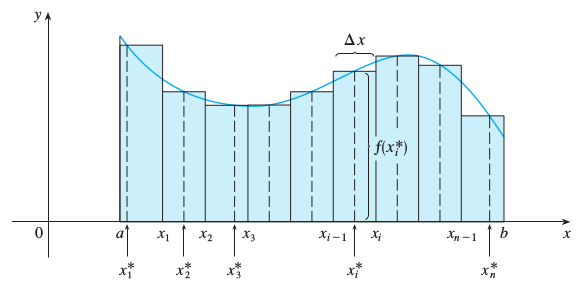
\includegraphics[scale=0.5]{imagens/int01.png}}\\
    \footnotesize{James Stewart: \emph{Cálculo} (8ª ed.,\ vol.\ 2,
      pg.\ 884)}
  \end{center}
\end{figure}

Sabemos que uma aproximação da área sob a função pode ser feita
com o seguinte procedimento:

\begin{enumerate}
  \item Dividimos o intervalo $a \le x \le b$ em $n$ intervalos
    menores iguais, $\Delta x$. Esse intervalo formará a base
    de um retângulo que será utilizado para estimar a área sob a
    função.
  \item Dentro de cada intervalo (de cada retângulo) $\Delta x$
    escolhemos um ponto de amostragem $x^*_i$ e calculamos a altura
    do retângulo, $f(x^*_i)$.
  \item A área de cada retângulo é dada então pela multiplicação de
    sua base ($\Delta x$) por sua altura ($f(x^*_i)$): área de cada
    retângulo é igual a $f(x^*_i) \Delta x$.
  \item A aproximação da área total sob a função $y = f(x)$ no
    intervalo $a \le x \le b$ é dada pela \emph{soma} das áreas de
    todos os retângulos, conforme a equação~\ref{eq:areaaprox}.
\end{enumerate}

\begin{equation}
  \label{eq:areaaprox}
  A \approx \sum_{i=1}^n f(x_i^*) \Delta x
\end{equation}
    
É fácil perceber que à medida em que dividimos o intervalo em um maior
número $n$ de retângulos (à medida em que diminuímos $\Delta x$), a
aproximação da área será melhor. No limite, quando $n$ tende ao
infinito, a área sob a curva tende ao valor exato e essa é a idéia do
cálculo integral (equação~\ref{eq:areaexata}):

\begin{equation}
  \label{eq:areaexata}
  \begin{split}
    A  &= \lim_{n \to \infty} \sum_{i=1}^n f(x_i^*) \Delta x\\
       &= \int_a^b f(x) \diff x
  \end{split}
\end{equation}


\subsection{Integrais duplas e o cálculo de volumes}
\label{sec:revisao-int2}
Uma expansão natural do problema do cálculo de áreas é o problema do
cálculo de \emph{volumes}, ou seja: dada uma função $z = f(x,y)$
qualquer, qual é o volume que está sob a função quando $x$ varia no
intervalo $a \le x \le b$ e $y$ varia no intervalo $c \le y \le d$
(ver figura~\ref{fig:volume1} abaixo):

\begin{figure}[H]
  \begin{center}
    \caption{O problema do cálculo do volume}
    \label{fig:volume1}
    \fbox{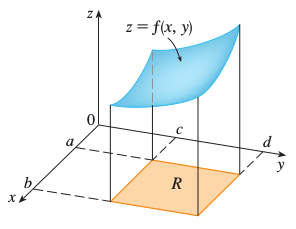
\includegraphics[scale=0.7]{imagens/int02.png}}\\
    \footnotesize{James Stewart: \emph{Cálculo} (8ª ed.,\ vol.\ 2,
      pg.\ 884)}
  \end{center}
\end{figure}

Como calcular o volume do sólido sob a função ilustrada na figura
anterior? Note que a variação no eixo $x$ e a variação no eixo $y$
delimitam uma ``base'' retangular $R$ sob a função $z = f(x,y)$. Isso
nos permite expandir o raciocínio do cálculo de áreas e obter uma
aproximação do volume com o seguinte procedimento (ver também
figura~\ref{fig:volume2} a seguir):

\begin{enumerate}
  \item Dividimos a base retangular $R$ em vários retângulos menores,
    $R_{ij}$
  \item A \emph{área de cada retângulo} $R_{ij}$ é então: $\Delta A = \Delta
    x \Delta y$    
  \item Dentro de cada retângulo $R_{ij}$ escolhemos um ponto de
    amostragem $(x^*_{ij}, y^*_{ij})$ e usamos esse ponto para
    calcular a altura do prisma, dada por: $f(x^*_{ij}, y^*_{ij})$
  \item O \emph{volume de cada prisma}, $V_{R_{ij}}$, é dado então pela multiplicação da
    área de sua base, $\Delta A$, por sua altura, $f(x^*_{ij},
    y^*_{ij})$, da seguinte maneira:
    \begin{equation}
      V_{R_{ij}} \approx f(x^*_{ij}, y^*_{ij}) \Delta A
    \end{equation}
\end{enumerate}

\begin{figure}[H]
  \begin{center}
    \caption{Dividindo o sólido sob a função em prismas}
    \label{fig:volume2}
    \fbox{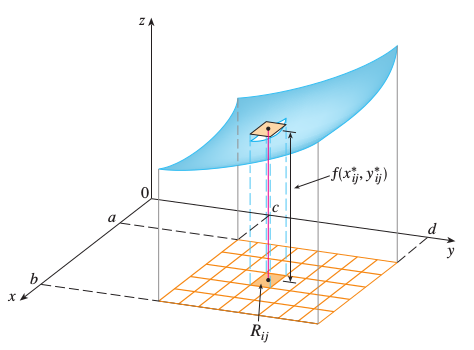
\includegraphics[scale=0.5]{imagens/int03.png}}\\
    \footnotesize{James Stewart: \emph{Cálculo} (8ª ed.,\ vol.\ 2,
      pg.\ 885)}
  \end{center}
\end{figure}

Para obter a estimativa do volume total sob a função, basta então
somar os volumes de todos os prismas (ver figura~\ref{fig:volume3}
e equação~\ref{eq:volumeaprox}):

\begin{figure}[H]
  \begin{center}
    \caption{Estimativa do volume sob a função}
    \label{fig:volume3}
    \fbox{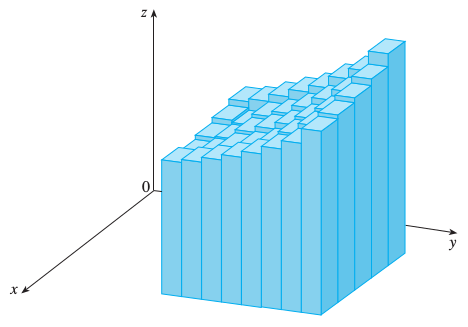
\includegraphics[scale=0.5]{imagens/int04.png}}\\
    \footnotesize{James Stewart: \emph{Cálculo} (8ª ed.,\ vol.\ 2,
      pg.\ 885)}
  \end{center}
\end{figure}

\begin{equation}
  \label{eq:volumeaprox}
  V \approx \sum_{i=1}^m \sum_{j=1}^n f(x_{ij}^*, y_{ij}^*) \Delta A
\end{equation}

Note que à medida em que dividimos o volume sob a função em um maior
número de prismas (maior número de retângulos $R_{ij}$, com intervalos
$\Delta x$ e $\Delta y$ menores e, portanto, com áreas $\Delta A$
menores), a aproximação do volume será melhor (ver
figura~\ref{fig:volume4}, a seguir):

\begin{figure}[H]
  \begin{center}
    \caption{Melhorando a estimativa do volume}
    \label{fig:volume4}
    \fbox{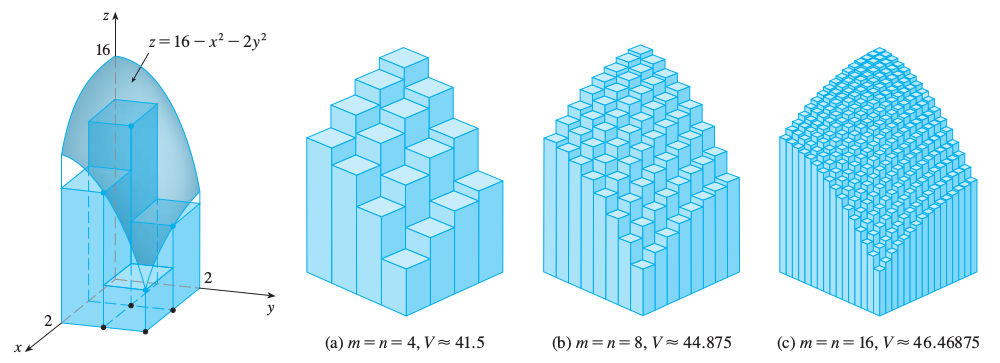
\includegraphics[scale=0.4]{imagens/int05_06.png}}\\
    \footnotesize{James Stewart: \emph{Cálculo} (8ª ed.,\ vol.\ 2,
      pg.\ 885)}
  \end{center}
\end{figure}

No limite, quanto o número de prismas tende ao infinito, o volume sob
a curva tende ao valor exato, e essa é a idéia do uso de integrais
duplas para o cálculo de volumes (equação~\ref{eq:volumeexato}):

\begin{equation}
  \label{eq:volumeexato}
  \begin{split}
      V &= \lim_{m, n \to \infty} \sum_{i=1}^m \sum_{j=1}^n f(x_{ij}^*,
      y_{ij}^*) \Delta A\\
        &= \iint\displaylimits_R f(x, y) \diff A\\
        &= \int_a^b \int_c^d f(x, y) \diff y \diff x
  \end{split}
\end{equation}

\section{Volumes com cálculo complicado}
\label{sec:volumes-dificeis}

O uso de integrais duplas para o cálculo de volumes (ver
equação~\ref{eq:volumeexato}) é aplicável em diversas situações e
em diferentes funções. Entretanto, existem funções nas quais o cálculo do
volume é difícil. Considere, por exemplo, o cálculo do volume do
sólido limitado abaixo pelo plano $z = 0$ e acima pelo parabolóide $z
= 1 - x^2 - y^2$ (figura~\ref{fig:voldif}):

\begin{figure}[H]
  \begin{center}
    \caption{Como calcular esse volume?}
    \label{fig:voldif}
    \fbox{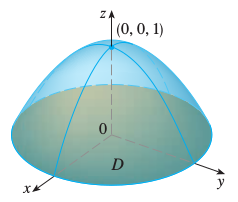
\includegraphics[scale=0.7]{imagens/int07.png}}\\
    \footnotesize{James Stewart: \emph{Cálculo} (8ª ed.,\ vol.\ 2,
      pg.\ 906)}
  \end{center}
\end{figure}

Note que a base não é mais um retângulo, é um disco $D$. Se tentarmos
calcular o volume através da utilização direta da
equação~\ref{eq:volumeexato}, chegaremos em uma expressão muito
difícil de resolver:

\begin{equation*}
    \begin{split}
      V &= \iint\displaylimits_D (1-x^2-y^2) \diff A\\
        &= \int_{-1}^1 \int_{-\sqrt{1-x^2}}^{\sqrt{1-x^2}}(1-x^2-y^2)
      \diff y \diff x
    \end{split}
\end{equation*}

E por que é difícil calcular o volume de funções parecidas com a
ilustrada na figura~\ref{fig:voldif}? Pois a ``base'' do sólido não é
mais um retângulo, é um disco, e, já que estamos utilizando o sistema
de \emph{coordenadas retangulares}, não é possível descrever o disco $D$ formado
por $x$ e $y$ por uma única função (ver figura~\ref{fig:voldif2}):

\begin{figure}[H]
  \begin{center}
    \caption{O disco $D$ não pode ser descrito por uma única função}
    \label{fig:voldif2}
    \fbox{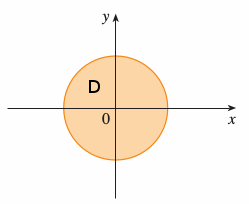
\includegraphics[scale=0.7]{imagens/int08.png}}\\
    \footnotesize{James Stewart: \emph{Cálculo} (8ª ed.,\ vol.\ 2,
      pg.\ 904)}
  \end{center}
\end{figure}

Para poder calcular esses volumes difíceis temos que mudar nosso ponto
de vista\footnote{Uma animação interessante que mostra como mudar o
  ponto de vista muda nosso entendimento sobre uma função pode ser
  vista em \url{http://www.youtube.com/watch?v=Dmc3mQ87GiQ}.}:
precisamos sair do sistema de coordenadas retangulares e
utilizar o sistema de \emph{coordenadas polares}.

A próxima seção explicará o que é o sistema de coordenadas polares
para, a partir desse conhecimento, demonstrar como o cálculo integral
pode ser feito utilizando-se esse referencial.

\section{O sistema de coordenadas polares}
\label{sec:coordpolar}

Um \emph{sistema de coordenadas} serve para representar a \emph{localização}
de um ponto no plano, através de um \emph{par ordenado} de números
chamados de \emph{coordenadas}.

Usualmente, quando representamos um ponto no plano, estamos nos
referindo ao \textbf{sistema de coordenadas retangulares}
(cartesianas), que são distâncias orientadas a partir de dois eixos
perpendiculares.

No sistema de coordenadas retangulares a localização de um ponto
$P$ é dada por

\begin{equation}
  P = (a, b)
\end{equation}

\noindent onde $a$ é a projeção de $P$ no eixo $x$, e $b$ é a projeção de $P$ no
eixo $y$.

Entretanto, para descrever curvas que exibem uma espécie de ``afinidade especial
por um ponto de origem'', como um círculo ou a trajetória de um
planeta ao longo de sua órbita, é melhor utilizar um outro sistema de
coordenadas, o sistema de coordenadas polares.

No \textbf{sistema de coordenadas polares} uma curva é descrita como a
trajetória de um ponto móvel cuja posição é especificada pela sua
\emph{direção a partir da origem} e pela sua \emph{distância até a
  origem}. Assim, qualquer ponto é localizado através de sua
\emph{direção} e sua \emph{distância} em relação à origem
(figura~\ref{fig:eixopolar}):

\begin{figure}[H]
  \begin{center}
    \caption{O eixo polar}
    \label{fig:eixopolar}
    \fbox{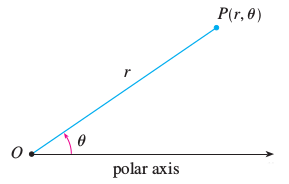
\includegraphics[scale=0.85]{imagens/int10.png}}\\
    \footnotesize{James Stewart: \emph{Cálculo} (8ª ed.,\ vol.\ 2,
      pg.\ 596)}
  \end{center}
\end{figure}

A direção é dada pelo ângulo $\theta$ em relação ao eixo polar
(geralmente em \emph{radianos}), e a distância $r$ é a distância
direta da origem até o ponto.

Esses dois números, $r$ e $\theta$,
são o par ordenado que formam as \emph{coordenadas polares} da
localização de um ponto no plano.

Por convenção, o par de coordenadas
polares é escrito primeiro informando-se a distância, e depois o ângulo:

\begin{equation}
  P = (r, \theta)
\end{equation}

Note o seguinte (figura~\ref{fig:caracteristicaspolar}):

\begin{itemize}[noitemsep]
  \item Esqueça o pensamento cartesiano de esquerda/direita (eixo $x$)
    e acima/abaixo (eixo $y$).
  \item Pense em termos de \emph{ao redor} e de
    \emph{distância} em relação ao \emph{polo}, a origem.
  \item $r = 0$ especifica a origem, independente de $\theta$.
  \item Cada ponto tem muitos pares de coordenadas polares, pois
    qualquer múltiplo de $2\pi$ adicionado ou subtraído de $\theta$
    faz uma ``volta completa'' na direção, parando no mesmo ponto.
  \item Cada coordenada polar define exatamente um ponto.
  \item Se aumentarmos $\theta$ por $\pi$, estamos na mesma ``reta''
    mas na direção contrária:
    \begin{equation}
      (r, \theta + \pi) = (-r, \theta)
    \end{equation}
\end{itemize}

\begin{figure}[H]
  \begin{center}
    \caption{Particularidades das coordenadas polares}
    \label{fig:caracteristicaspolar}
    \fbox{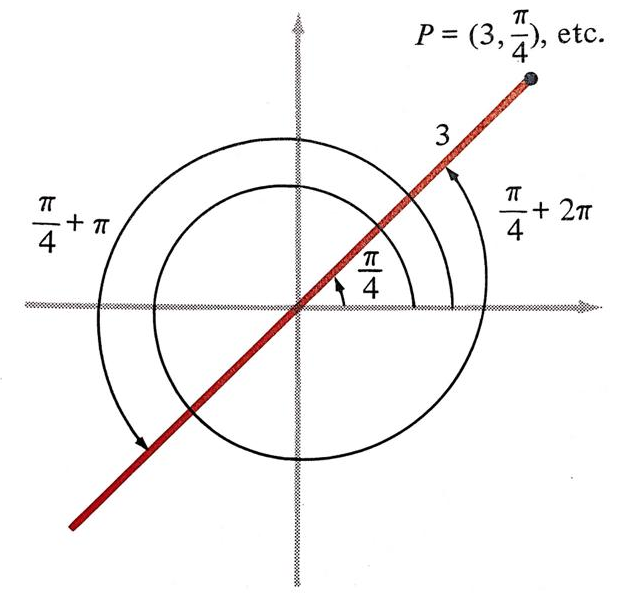
\includegraphics[scale=0.3]{imagens/int11.png}}\\
    \footnotesize{George Simmons: \emph{Calculus with Analytic
            Geometry} (2ª ed.,\ pg.\ 560)}
  \end{center}
\end{figure}

Uma representação interessante do sistema de coordenadas polares e de
como os pontos são localizados é
exibida nas figuras~\ref{fig:sistpolar} e \ref{fig:sistpolar2}, abaixo:

\begin{figure}[H]
  \begin{center}
    \caption{O sistema de coordenadas polares}
    \label{fig:sistpolar}
    \fbox{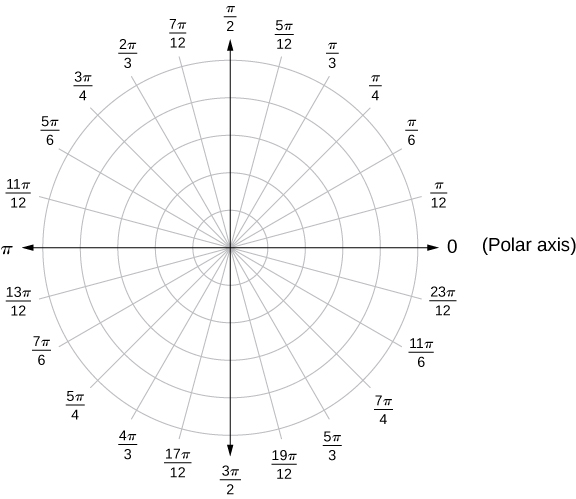
\includegraphics[scale=0.8]{imagens/int16.jpg}}\\
    \footnotesize{Gilbert Strang \& Edwin Herman: \emph{Calculus}
          (ed.\ online, 2017, vol.\ 2, pg.\ 645)}
  \end{center}
\end{figure}

\begin{figure}[H]
   \begin{center}
     \caption{Os pontos estão ao redor da origem}
     \label{fig:sistpolar2}
     \fbox{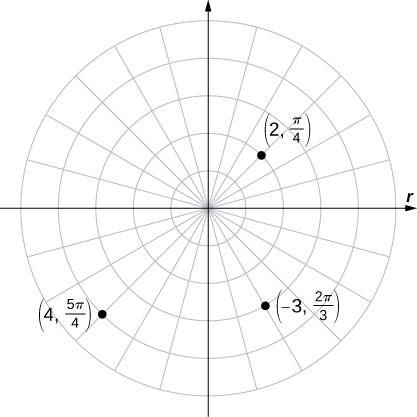
\includegraphics[scale=0.9]{imagens/int17.jpg}}\\
     \footnotesize{Gilbert Strang \& Edwin Herman: \emph{Calculus}
          (ed.\ online, 2017, vol.\ 2, pg.\ 646)}
     \end{center}
\end{figure}



\subsection{Equações e curvas polares}
\label{sec:coordpolar-eqcurv}

Para ilustrar de modo cristalino como uma mesma função pode ser
entendida de forma diferente dependendo do sistema de coordenadas
utilizado (retangular ou polar), considere a seguinte função: $r =
\cos(2\theta)$. Se essa função for plotada em coordenadas
retangulares, será uma onda; se for plotada em coordenadas polares
será uma rosa (figura~\ref{fig:mesmafuncdifview}):

\begin{figure}[H]
    \begin{center}
      \caption{Mesma função, dois pontos de vista}
      \label{fig:mesmafuncdifview}
      \fbox{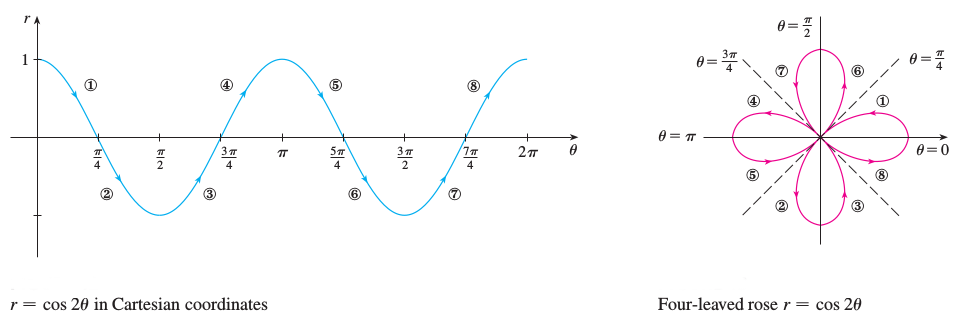
\includegraphics[scale=0.45]{imagens/int15.png}}\\
      \footnotesize{James Stewart: \emph{Cálculo} (8ª ed.,\ vol.\ 2, pg.\ 600)}
    \end{center}
\end{figure}

O gráfico de uma equação polar $r = f(\theta)$ ou, mais genericamente,
$F(r,\theta)=0$, consiste de todos os pontos $P$ que têm \emph{pelo
  menos uma} representação $(r, \theta)$ cujas coordenadas satisfaçam
a equação polar. Isso faz com que as equações polares, quando
plotadas, assumam formas belas e inusitadas (ver figuras:
\ref{fig:belo1}, \ref{fig:belo2}, \ref{fig:belo3}, \ref{fig:belo4},
\ref{fig:belo5}, \ref{fig:belo6}, \ref{fig:belo7}).

\begin{figure}[H]
  \begin{center}
    \caption{A beleza polar: espiral}
    \label{fig:belo1}
    \fbox{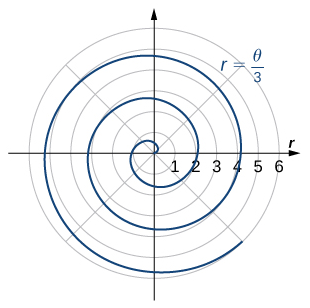
\includegraphics[scale=0.5]{imagens/int18.png}}\\
    \footnotesize{Gilbert Strang \& Edwin Herman: \emph{Calculus}
      (ed.\ online, 2017, vol.\ 2, pg.\ 651)}
  \end{center}
\end{figure}

\begin{figure}[H]
  \begin{center}
    \caption{A beleza polar: cardióde}
    \label{fig:belo2}
    \fbox{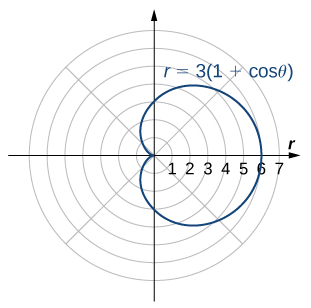
\includegraphics[scale=0.5]{imagens/int19.png}}\\
    \footnotesize{Gilbert Strang \& Edwin Herman: \emph{Calculus}
        (ed.\ online, 2017, vol.\ 2, pg.\ 652)}
  \end{center}
\end{figure}

\begin{figure}[H]
  \begin{center}
    \caption{A beleza polar: Limaçon}
    \label{fig:belo3}
    \fbox{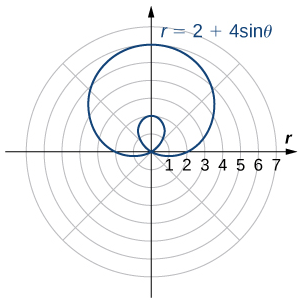
\includegraphics[scale=0.5]{imagens/int20.png}}\\
    \footnotesize{Gilbert Strang \& Edwin Herman: \emph{Calculus}
         (ed.\ online, 2017, vol.\ 2, pg.\ 652)}
  \end{center}
\end{figure}

\begin{figure}[H]
  \begin{center}
    \caption{A beleza polar: rosácea}
    \label{fig:belo4}
    \fbox{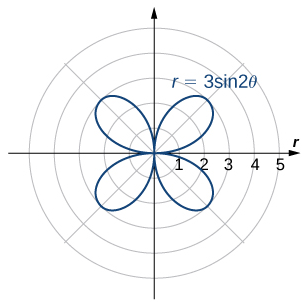
\includegraphics[scale=0.5]{imagens/int21.png}}\\
    \footnotesize{Gilbert Strang \& Edwin Herman: \emph{Calculus}
          (ed.\ online, 2017, vol.\ 2, pg.\ 652)}
  \end{center}
\end{figure}

\begin{figure}[H]
  \begin{center}
    \caption{A beleza polar: rosácea com 3 pétalas}
    \label{fig:belo5}
    \fbox{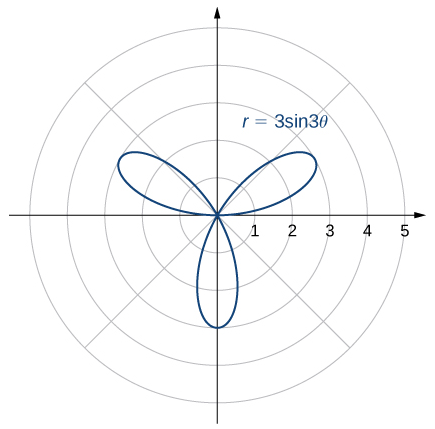
\includegraphics[scale=0.38]{imagens/int22.png}}\\
    \footnotesize{Gilbert Strang \& Edwin Herman: \emph{Calculus}
          (ed.\ online, 2017, vol.\ 2, pg.\ 652)}
  \end{center}
\end{figure}

\begin{figure}[H]
  \begin{center}
    \caption{A beleza polar: formas inusitadas}
    \label{fig:belo6}
    \fbox{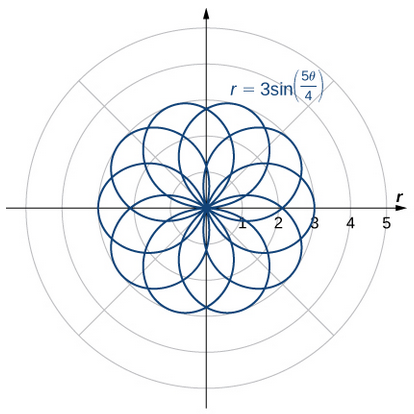
\includegraphics[scale=0.4]{imagens/int23.png}}\\
    \footnotesize{Gilbert Strang \& Edwin Herman: \emph{Calculus}
         (ed.\ online, 2017, vol.\ 2, pg.\ 652)}
  \end{center}
\end{figure}

\begin{figure}[H]
  \begin{center}
    \caption{A beleza polar: espiral logarítmica}
    \label{fig:belo7}
    \fbox{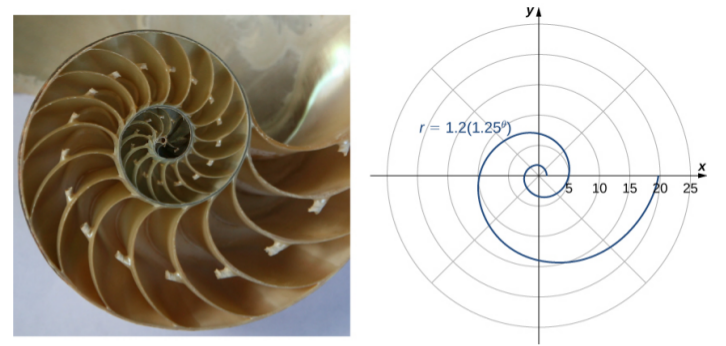
\includegraphics[scale=0.45]{imagens/int24.png}}\\
    \footnotesize{Gilbert Strang \& Edwin Herman: \emph{Calculus}
          (ed.\ online, 2017, vol.\ 2, pg.\ 655)}
  \end{center}
\end{figure}

Não é possível deixar de notar, pela figura~\ref{fig:belo7}, como uma
simples função matemática, $r = 1.2(1.25^\theta)$, pode ser utilizada
para descrever uma obra de Deus, uma obra da criação. Isso nos faz
pensar que Galileu Galilei estava correto ao dizer que ``a matemática
é o alfabeto que Deus usou para escrever o universo''\footnote{Apesar
  de universalmene conhecida e atribuída à Galileu, sabe-se que ele
  não escreveu exatamente isso. Uma simples pesquisa na internet
  mostrará diversas citações semelhantes e polêmicas quanto a versão
  exata ou correta da frase.}.


\subsection{De retangular para polar e vice-versa}
\label{sec:coordpolar-equiv}

Como uma mesma função pode ser expressa tanto em coordenadas
retangulares quanto em coordenadas polares, existe um modo direto de
transformar coordenadas retangulares em polares e vice-versa
(figura~\ref{fig:retpol}) utilizando-se trigonometria:

\begin{figure}[H]
  \begin{center}
    \caption{Retangular $\leftrightarrows$ Polar}
    \label{fig:retpol}
    \fbox{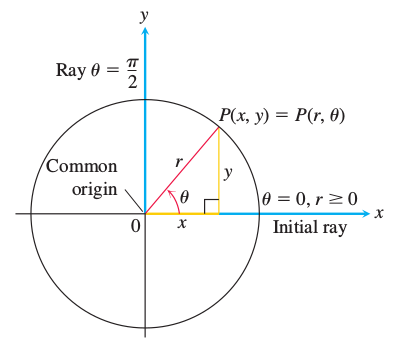
\includegraphics[scale=0.6]{imagens/int25.png}}\\
    \footnotesize{George Thomas: \emph{Thomas' Calculus: early transcedentals}
          (14ª ed., 2017, pg.\ 683)}
  \end{center}
\end{figure}

A transformação de coordenadas polares em coordenadas retangulares
é dada por:

\begin{equation}
  x = r \cos(\theta)
\end{equation}
\begin{equation}
  y = r \sin(\theta)
\end{equation}

E a transformação de coordenadas retangulares em coordenadas polares é
dada por (cuidado para que o sinal de $r$ e a escolha de $\theta$
sejam consistentes com o quadrante no qual o ponto $(x, y)$ está):

\begin{equation}
  r^2 = x^2 + y^2
\end{equation}
\begin{equation}
  \tan(\theta) = \frac{y}{x} \quad \therefore \quad \theta = \arctan\left(\frac{y}{x}\right)
\end{equation}

Essas transformações entre coordenadas retangulares e polares serão
fundamentais para o cálculo do volume utilizando-se integrais.

\section{Integrais simples em coordenadas polares}
\label{sec:int1polar}

O problema do cálculo de áreas examinado na
seção~\ref{sec:revisao-int1}, com coordenadas retangulares, tem um
equivalente em coordenadas polareas, ou seja: dada uma equação polar
qualquer $r = f(\theta)$, como encontrar a área da região $R$
delimitada pelos ângulos $\theta = a$ e $\theta = b$
(figura~\ref{fig:areapolar1})?

\begin{figure}[H]
  \begin{center}
    \caption{O problema da área em coordenadas polares}
    \label{fig:areapolar1}
    \fbox{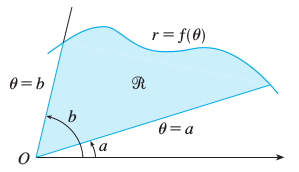
\includegraphics[scale=0.7]{imagens/int26.png}}\\
    \footnotesize{James Stewart: \emph{Cálculo} (8ª ed.,\ vol.\ 2, pg.\ 606)}
  \end{center}
\end{figure}

A solução é dividir a região $R$ em vários setores, calcular a área de
cada setor e somar todas as áreas (figura~\ref{fig:areapolar2}), de
forma análoga ao procedimento para o cálculo de áreas em coordenadas
retangulares:

\begin{figure}[H]
  \begin{center}
    \caption{Divisão da região $R$ em vários setores}
    \label{fig:areapolar2}
    \fbox{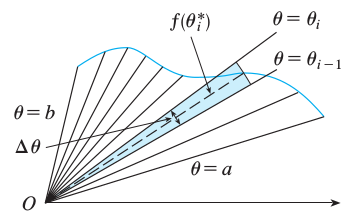
\includegraphics[scale=0.6]{imagens/int27.png}}\\
    \footnotesize{James Stewart: \emph{Cálculo} (8ª ed.,\ vol.\ 2, pg.\ 606)}
  \end{center}
\end{figure}

Sabemos que a área de um setor de um círculo é proporcional ao
ângulo $\theta$ (figura~\ref{fig:areapolar3}) e dada por:

\begin{equation}
  \label{eq:areasetor}
  \begin{split}
    A &= \pi r^2 \times \frac{\theta}{2\pi}\\
    &= \frac{1}{2}\theta r^2
  \end{split}
\end{equation}

\begin{figure}[H]
  \begin{center}
    \caption{Área de um setor de um círculo}
    \label{fig:areapolar3}
    \fbox{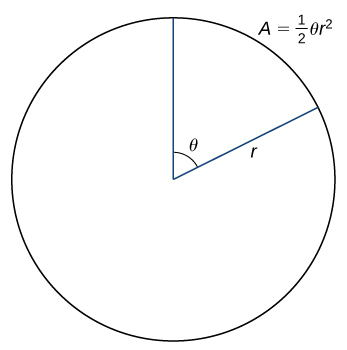
\includegraphics[scale=0.45]{imagens/int28.png}}\\
    \footnotesize{Gilbert Strang \& Edwin Herman: \emph{Calculus}
          (ed.\ online, 2017, vol.\ 2, pg.\ 663)}
    \end{center}
\end{figure}

Como o raio $r$ na equação~\ref{eq:areasetor} corresponde à
$f(\theta^*_i)$, podemos calcular a área de \emph{cada
setor} na figura~\ref{fig:areapolar2} da seguinte forma:

\begin{equation}
  \begin{split}
    \Delta A_i &\approx \frac{1}{2}\color{red}r\color{black}^2 \Delta \theta\\
        &\approx \frac{1}{2}\left[\color{red}f(\theta_i^*)\color{black}\right]^2 \Delta \theta
  \end{split}
\end{equation}

Para calcular a estimativa da área total da região $R$ sob a função $r = f(\theta)$,
delimitada pelos ângulos $\theta = a$ e $\theta =  b$, basta somar as
áreas de cada setor individual:

\begin{equation}
    A \approx \sum_i^n \frac{1}{2}\left[f(\theta_i^*)\right]^2 \Delta \theta
\end{equation}

É fácil perceber que à medida em que aumentamos o números de setores a
estimativa do cálculo da área fica mais precisa. No limite, quando o
número de setores tende ao infinito, a área tende ao valor exato, e
essa é a idéia do cálculo de áreas em coordenadas polares:

\begin{equation}
  \begin{split}
  A &= \lim_{n \to \infty} \sum_i^n
  \frac{1}{2}\left[f(\theta_i^*)\right]^2 \Delta \theta\\
  &= \int_a^b \frac{1}{2}\left[f(\theta)\right]^2 \diff \theta\\
  &= \int_a^b \frac{1}{2}r^2 \diff \theta
  \end{split}
\end{equation}

\section{Integrais duplas em coordenadas polares}
\label{sec:int2polar}

Tendo como base o conhecimento acumulado nas seções anteriores, agora
é possível expandir o problema do cálculo de área em coordenadas
polares para o problema do volume em coordenadas polares.

Revisitando o problema do cálculo do volume do sólido limitado abaixo
pelo plano $z = 0$ e acima pelo parabolóide $z = 1 - x^2 - y^2$ (ver
figura~\ref{fig:voldif} na página~\pageref{fig:voldif}),
utilizaremos um artifício para dividir a
base do sólido (o disco $D$) em diversos \emph{retângulos polares} e, a
partir desses retângulos, faremos o cálculo do volume.

Um \textbf{retângulo polar} (figura~\ref{fig:retangpolar}) é a região
formada pelo conjunto de coordenadas polares delimitadas por dois
ângulos e duas distâncias:

\begin{equation}
R = \{(r,\theta)\, | \, a \le r \le b,
\alpha \le \theta \le \beta\}
\end{equation}

\begin{figure}[H]
  \begin{center}
    \caption{O retângulo polar}
    \label{fig:retangpolar}
    \fbox{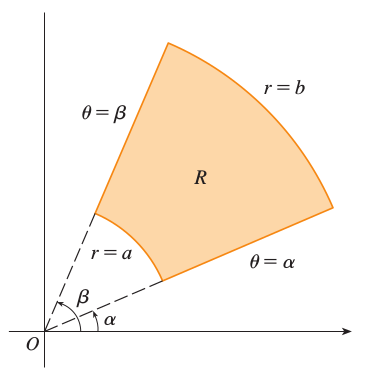
\includegraphics[scale=0.45]{imagens/int29.png}}\\
    \footnotesize{James Stewart: \emph{Cálculo} (8ª ed.,\ vol.\ 2, pg.\ 904)}
  \end{center}
\end{figure}

Usando o conceito de retângulos polares, dividimos a base do sólido (o
disco $D$ na figura~\ref{fig:voldif}) em vários retângulos polares,
conforme ilustrado na figura~\ref{fig:retangpolar2} a seguir, com as
seguintes características:

\begin{itemize}
  \item O intervalo $[a, b]$ é dividido em $m$ intervalos $[r_{i-1},
    r_i]$, de larguras \emph{iguais}:
    \begin{equation*}
      \Delta r = \frac{b-a}{m}
    \end{equation*}
  \item O intervalo $[\alpha, \beta]$ é dividido em $n$ intervalos
    $[\theta_{j-1}, \theta_j]$, de larguras \emph{iguais}:
    \begin{equation*}
      \Delta \theta = \frac{\beta - \alpha}{n}
    \end{equation*}
  \item O centro de cada retângulo polar é dado por:
    \begin{equation*}
      r_i^* = \frac{1}{2}(r_{i-1}+r_i) \quad\ \quad\ \text{ e }
      \quad\ \quad\ \theta_j^* = \frac{1}{2}(\theta_{j-1}+\theta_j)
    \end{equation*}
\end{itemize}

\begin{figure}[H]
  \begin{center}
    \caption{Divisão da base do sólido em retângulos polares}
    \label{fig:retangpolar2}
    \fbox{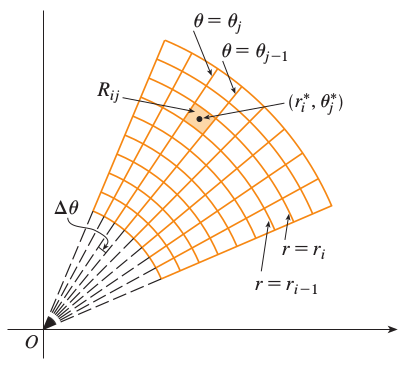
\includegraphics[scale=0.45]{imagens/int30.png}}\\
    \footnotesize{James Stewart: \emph{Cálculo}\\ (8ª ed.,\ vol.\ 2, pg.\ 904)}
  \end{center}
\end{figure}

Podemos então calcular a área de \emph{cada retângulo polar} usando a
equação~\ref{eq:areasetor} da seguinte maneira:

\begin{equation}
  \label{eq:arearetangpolar}
  \begin{split}
    \Delta A_i &= \left(\frac{1}{2} r_i^2\Delta \theta\right) - \left(\frac{1}{2} r_{i-1}^2\Delta \theta\right)\\
               &= \frac{1}{2}(r_i^2 - r_{i-1}^2)\Delta \theta\\
               &= \ldots\\
               &= \color{red}r_i^*\color{black} \Delta r \Delta \theta
  \end{split}
\end{equation}

Note que na equação~\ref{eq:arearetangpolar}, que calcula a área de
cada retângulo polar, surgiu um fator $r_i^*$ que multiplica $\Delta r
\Delta \theta$. Esse fator é necessário para levar em conta que
retângulos mais distantes da origem terão área maior (do contrário,
como dividimos os setores em larguras iguais, todos os retângulos
teriam a mesma área, o que não faz sentido\footnote{Um vídeo
  disponível em uma página da Universidade do Texas fornece uma
  explicação interessante para isso:
  \url{https://web.ma.utexas.edu/users/m408m/Display15-4-2.shtml}}).

Agora que já sabemos como calcular a área de cada retângulo polar da
base de nosso sólido, vamos expandir o raciocínio para o volume do
prisma que tem como base o retângulo polar e altura até a superfície
da função, conforme ilustrado na figura~\ref{fig:prismapolar} a
seguir:

\begin{figure}[H]
  \begin{center}
    \caption{Volume do sólido que tem como base o retângulo polar}
    \label{fig:prismapolar}
    \fbox{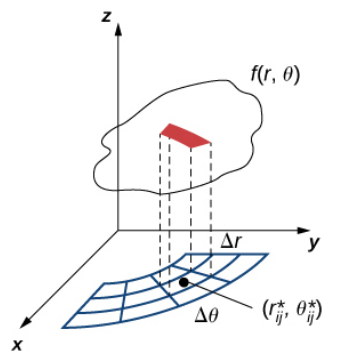
\includegraphics[scale=0.5]{imagens/int31.png}}\\
    \footnotesize{Gilbert~Strang~\&~Edwin~ Herman:\\ \emph{Calculus}
        (ed.\ online, 2017, vol.\ 3, pg.\ 527)}
  \end{center}
\end{figure}

O volume de cada prisma será dado pela multiplicação da área de sua base,
$\Delta A_i$, com sua altura, dada em coordenadas polares por $f[r_i^*
  \cos(\theta_j^*), r_i^* \sin(\theta_j^*)]$:

\begin{equation}
      V_{R_{ij}} \approx f[r_i^* \cos(\theta_j^*), r_i^* \sin(\theta_j^*)] \Delta A_i
\end{equation}

E a estimativa do volume total sob o sólido é dada pela somatória do
volume individual de todos os prismas:

\begin{equation}
  \begin{split}
    V &\approx \sum_{i=1}^m \sum_{j=1}^n f[r_i^* \cos(\theta_j^*),
    r_i^* \sin(\theta_j^*)] \Delta A_i\\
      &\approx \sum_{i=1}^m \sum_{j=1}^n f[r_i^* \cos(\theta_j^*),
    r_i^* \sin(\theta_j^*)] \color{red}r_i^*\color{black}\Delta r
    \Delta \theta
  \end{split}
\end{equation}

Perceba que à medida em que aumentamos o número de prismas (à medida
em que os retângulos polares ficam menores), a estimativa do cálculo
do volume fica mais precisa. No limite, quando o número de retângulos
polares tendo ao infinito, o volume tende ao valor exato, e essa é a
idéia de usar coordenadas polares para o cálculo de volumes:

\begin{equation}
  \begin{split}
    V &= \lim_{m,n \to \infty} \sum_{i=1}^m \sum_{j=1}^n f[r_i^* \cos(\theta_j^*),
      r_i^* \sin(\theta_j^*)] \Delta A_i\\
      &= \iint\displaylimits_R f[r \cos(\theta), r \sin(\theta)]
    \diff A\\
      &= \int_\alpha^\beta \int_a^b f[r \cos(\theta), r
      \sin(\theta)] \color{red}r\color{black} \diff r \diff \theta
  \end{split}
\end{equation}

Em resumo, quando temos uma função de difícil integração quando
expressa em coordenadas retangulares, $\displaystyle \int_a^b \int_c^d f(x, y) \diff
y \diff x$,
podemos reexpressar a mesma função em coordenadas polares,
$\displaystyle \int_\alpha^\beta \int_a^b f[r \cos(\theta), r
      \sin(\theta)] r \diff r \diff \theta$,
para facilitar o cálculo.



%%%%%%%%%%%%%%%%%%%%%%%%%%%%%%%%%%%%%%%%%%%%%%%%%%%%%%%%%%%%%%%%%%%%%%%%%%%%%%%%
%%% Apêndices
\appendix
\section{Bibliografia consultada}
\label{sec:biblio}

\begin{itemize}
  \item James Stewart: \emph{Cálculo}, 8ª edição, volume 2 (seções
    10.3, 10.4, 15.3)
  \item George F.\ Simmons: \emph{Calculus with Analytic Geometry},
    2ª edição (seções 16.1, 16.2, 16.3, 20.4)
  \item George B.\ Thomas, JR: \emph{Thomas' Calculus: early
    transcedentals}, 14ª (seções 11.3, 11.4, 11.5, 15.4)
  \item Gilbert Strang \& Edwin ``Jed'' Herman: \emph{Calculus},
    edição online de 2017, volume 2 (seções 7.3, 7.4)
  \item Gilbert Strang \& Edwin ``Jed'' Herman: \emph{Calculus},
    edição online de 2017, volume 3 (seções 1.3, 1.4, 5.3)
  \item Mauri C.\ Nascimento. \emph{Coordenadas Polares.}. Dep. de Matemática, Unesp/Bauru.
    Disponível online em \url{http://wwwp.fc.unesp.br/~mauri/Down/Polares.pdf}.
  \item Bosco Nogueira. \emph{Integrais Duplas}. Departamento de Matemática, UFPB.
    Disponível online em \url{http://www.mat.ufpb.br/bosco/calculoiii2011/nciii.pdf}
  \item Lorenzo Sadun. \emph{Double Integrals in Poolar Coordinates}. M408M, Texas University Learning Module Pages.
    Disponível online em \url{https://web.ma.utexas.edu/users/m408m/Display15-4-2.shtm}
\end{itemize}


\section{Integrantes do Grupo 1}
\label{sec:grupo}

\begin{itemize}
  \item Abrantes Araújo Silva Filho
  \item Alecsandro Queiroz
  \item Anderson Kirmse Rodrigues
  \item Anna Karolyna Lima Santos
  \item Antônio Carlos da Silva Alberto
  \item Beatriz Sauvalaio Benezolli
  \item Braian dos Santos Calot
  \item Bruno Brasil Ferreira
  \item Bryan Lucas Barbosa Lima
  \item Danielle Marcelino Cicilioti
\end{itemize}


\section{Fontes em \LaTeX}
\label{sec:fontes}

Este trabalho (juntamente com os slides para apresentação) foram escritos
utilizando-se \TeX\ e \LaTeX. O código fonte deste trabalho está disponível
online para estudantes interessados em aprender a utilizar essas ferramentas em:
\url{https://github.com/abrantesasf/matematica/tree/master/calculus/faesa/calculo3/polar}



%%%%%%%%%%%%%%%%%%%%%%%%%%%%%%%%%%%%%%%%%%%%%%%%%%%%%%%%%%%%%%%%%%%%%%%%%%%%%%%%
%%% Back matter
\bibliography{utils/biblioteca}

\printindex


%%%%%%%%%%%%%%%%%%%%%%%%%%%%%%%%%%%%%%%%%%%%%%%%%%%%%%%%%%%%%%%%%%%%%%%%%%%%%%%%
%%% Termina o documento
\end{document}
